\documentclass[11pt]{article}

\usepackage{times}
\usepackage{epsf}
\usepackage{epsfig}
\usepackage{amsmath, alltt, amssymb, xspace}
\usepackage{wrapfig}
\usepackage{fancyhdr}
\usepackage{url}
\usepackage{verbatim}
\usepackage{fancyvrb}

\usepackage{subfigure}
\usepackage{cite}
%\usepackage{cases}
%\usepackage{ltexpprt}
%\usepackage{verbatim}

%\topmargin      -0.70in  % distance to headers
%\headheight     0.2in   % height of header box
%\headsep        0.4in   % distance to top line
%\footskip       0.3in   % distance from bottom line

% Horizontal alignment
\topmargin      -0.50in  % distance to headers
\oddsidemargin  0.0in
\evensidemargin 0.0in
\textwidth      6.5in
\textheight     8.9in 


%\centerfigcaptionstrue

%\def\baselinestretch{0.95}


\newcommand\discuss[1]{\{\textbf{Discuss:} \textit{#1}\}}
%\newcommand\todo[1]{\vspace{0.1in}\{\textbf{Todo:} \textit{#1}\}\vspace{0.1in}}
\newtheorem{problem}{Problem}[section]
%\newtheorem{theorem}{Theorem}
%\newtheorem{fact}{Fact}
\newtheorem{define}{Definition}[section]
%\newtheorem{analysis}{Analysis}
\newcommand\vspacenoindent{\vspace{0.1in} \noindent}

%\newenvironment{proof}{\noindent {\bf Proof}.}{\hspace*{\fill}~\mbox{\rule[0pt]{1.3ex}{1.3ex}}}
%\newcommand\todo[1]{\vspace{0.1in}\{\textbf{Todo:} \textit{#1}\}\vspace{0.1in}}

%\newcommand\reducespace{\vspace{-0.1in}}
% reduce the space between lines
%\def\baselinestretch{0.95}

\newcommand{\fixmefn}[1]{ \footnote{\sf\ \ \fbox{FIXME} #1} }
\newcommand{\todo}[1]{
\vspace{0.1in}
\fbox{\parbox{6in}{TODO: #1}}
\vspace{0.1in}
}

\newcommand{\mybox}[1]{
\vspace{0.2in}
\noindent
\fbox{\parbox{6.5in}{#1}}
\vspace{0.1in}
}


\newcounter{question}
\setcounter{question}{1}

\newcommand{\myquestion} {{\vspace{0.1in} \noindent \bf Question \arabic{question}:} \addtocounter{question}{1} \,}

\newcommand{\myproblem} {{\noindent \bf Problem \arabic{question}:} \addtocounter{question}{1} \,}


\newcommand{\copyrightnoticeA}[1]{
\vspace{0.1in}
\fbox{\parbox{6in}{\small Copyright \copyright\ 2006 - 2014\ \ Wenliang Du, Syracuse University.\\ 
      The development of this document is partially funded by 
      the National Science Foundation's Course, Curriculum, and Laboratory 
      Improvement (CCLI) program under Award No. 0618680 and 0231122. 
      Permission is granted to copy, distribute and/or modify this document
      under the terms of the GNU Free Documentation License, Version 1.2
      or any later version published by the Free Software Foundation.
      A copy of the license can be found at http://www.gnu.org/licenses/fdl.html.}}
\vspace{0.1in}
}


\newcommand{\copyrightnotice}[1]{
\vspace{0.1in}
\fbox{\parbox{6in}{\small Copyright \copyright\ 2006 - 2014\ \ Wenliang Du, Syracuse University.\\
      The development of this document is/was funded by three grants from
      the US National Science Foundation: Awards No. 0231122 and 0618680 from
      TUES/CCLI and  Award No. 1017771 from Trustworthy Computing.
      This lab was imported into the Labtainer framework by the Naval Postgraduate 
      School, Center for Cybersecurity and Cyber Operations under National Science 
      Foundation Award No. 1438893.
      Permission is granted to copy, distribute and/or modify this document
      under the terms of the GNU Free Documentation License, Version 1.2
      or any later version published by the Free Software Foundation.
      A copy of the license can be found at http://www.gnu.org/licenses/fdl.html.}}
\vspace{0.1in}
}

\newcommand{\copyrightnoticeB}[1]{
\vspace{0.1in}
\fbox{\parbox{6in}{\small Copyright \copyright\ 2006 - 2014\ \ Wenliang Du, Syracuse University.\\
      The development of this document is/was funded by the following grants from
      the US National Science Foundation: No. 0231122, 0618680, and 1303306.
      Permission is granted to copy, distribute and/or modify this document
      under the terms of the GNU Free Documentation License, Version 1.2
      or any later version published by the Free Software Foundation.
      A copy of the license can be found at http://www.gnu.org/licenses/fdl.html.}}
\vspace{0.1in}
}


\newcommand{\nocopyrightnotice}[1]{
\vspace{0.1in}
\fbox{\parbox{6in}{\small  
      The development of this document is funded by 
      the National Science Foundation's Course, Curriculum, and Laboratory 
      Improvement (CCLI) program under Award No. 0618680 and 0231122. 
      Permission is granted to copy, distribute and/or modify this document.
      }}
\vspace{0.1in}
}

\newcommand{\idea}[1]{
\vspace{0.1in}
{\sf IDEA:\ \ \fbox{\parbox{5in}{#1}}}
\vspace{0.1in}
}

\newcommand{\questionblock}[1]{
\vspace{0.1in}
\fbox{\parbox{6in}{#1}}
\vspace{0.1in}
}


\newcommand{\minix}{{\tt Minix}\xspace}
\newcommand{\unix}{{\tt Unix}\xspace}
\newcommand{\linux}{{\tt Linux}\xspace}
\newcommand{\ubuntu}{{\tt Ubuntu}\xspace}
\newcommand{\selinux}{{\tt SELinux}\xspace}
\newcommand{\freebsd}{{\tt FreeBSD}\xspace}
\newcommand{\solaris}{{\tt Solaris}\xspace}
\newcommand{\windowsnt}{{\tt Windows NT}\xspace}
\newcommand{\setuid}{{\tt Set-UID}\xspace}
%\newcommand{\smx}{{\tt Smx}\xspace}
\newcommand{\smx}{{\tt Minix}\xspace}
\newcommand{\relay}{{\tt relay}\xspace}
\newcommand{\isys}{{\tt iSYS}\xspace}
\newcommand{\ilan}{{\tt iLAN}\xspace}
\newcommand{\iSYS}{{\tt iSYS}\xspace}
\newcommand{\iLAN}{{\tt iLAN}\xspace}
\newcommand{\iLANs}{{\tt iLAN}s\xspace}
\newcommand{\bochs}{{\tt Bochs}\xspace}

\newcommand\FF{{\mathcal{F}}}

\newcommand{\argmax}[1]{
\begin{minipage}[t]{1.25cm}\parskip-1ex\begin{center}
argmax
#1
\end{center}\end{minipage}
\;
}

\newcommand{\bm}{\boldmath}
\newcommand  {\bx}    {\mbox{\boldmath $x$}}
\newcommand  {\by}    {\mbox{\boldmath $y$}}
\newcommand  {\br}    {\mbox{\boldmath $r$}}


%\pagestyle{fancyplain}
%\lhead[\thepage]{\thesection}      % Note the different brackets!
%\rhead[\thesection]{SEED Laboratories}
%\lfoot[\fancyplain{}{}]{Syracuse University} 
%\cfoot[\fancyplain{}{}]{\thepage} 

\newcommand{\tstamp}{\today}   
%\lhead[\fancyplain{}{\thepage}]         {\fancyplain{}{\rightmark}}
%\chead[\fancyplain{}{}]                 {\fancyplain{}{}}
%\rhead[\fancyplain{}{\rightmark}]       {\fancyplain{}{\thepage}}
%\lfoot[\fancyplain{}{}]                 {\fancyplain{\tstamp}{\tstamp}}
%\cfoot[\fancyplain{\thepage}{}]         {\fancyplain{\thepage}{}}
%\rfoot[\fancyplain{\tstamp} {\tstamp}]  {\fancyplain{}{}}

\pagestyle{fancy}
%\lhead{\bfseries Computer Security Course Project}
\lhead{\bfseries SEED Labs}
\chead{}
\rhead{\small \thepage}
\lfoot{}
\cfoot{}
\rfoot{}

\usepackage{listings}
\usepackage{color}

\definecolor{dkgreen}{rgb}{0,0.6,0}
\definecolor{gray}{rgb}{0.5,0.5,0.5}
\definecolor{mauve}{rgb}{0.58,0,0.82}

\lstset{frame=tb,
  language=C,
  aboveskip=3mm,
  belowskip=3mm,
  showstringspaces=false,
  columns=flexible,
  basicstyle={\small\ttfamily},
  numbers=none,
  numberstyle=\tiny\color{gray},
  keywordstyle=\color{blue},
  commentstyle=\color{dkgreen},
  stringstyle=\color{mauve},
  breaklines=true,
  breakatwhitespace=true,
  tabsize=3
}




%\documentclass{article} 
%\usepackage{graphicx}
%\usepackage{color}
%\usepackage[latin1]{inputenc}
%\usepackage{lgrind}
%\input {highlight.sty}
\usepackage{xspace}
\usepackage{graphics}
\usepackage{hyperref}

\newcommand{\ssh}{\textit{ssh}\xspace}
\newcommand{\scp}{\textit{scp}\xspace}
\newcommand{\ping}{\textit{ping}\xspace}
\newcommand{\base}{\textbf{base}\xspace}
\newcommand{\host}[1]{\textbf{host{#1}}\xspace}

% numbering verbatims
\newcounter{myverb}
\usepackage{verbatim}

\BeforeBeginEnvironment{verbatim}{%
  \\
  \refstepcounter{myverb}%
   \\
  \noindent\textbf{Command \themyverb:}
  }


\lhead{\bfseries SSH-TUNNEL }

\def \code#1 {\fbox{\scriptsize{\texttt{#1}}}}

\begin{document}

\begin{center}
{\LARGE SSH-TUNNEL LAB}
\end{center}

\vspace{0.1in}
\fbox{\parbox{6in}{\small
    This document was originally created by George
    W. Dinolt, \href{mailto:gwdinolt.@nps.edu}{gwdinolt@nps.edu}.
    Permission is granted to copy, distribute and or modify this
    document under the terms of the GNU Free Documentation License, Version 3.0
      or any later version published by the Free Software Foundation.
      A copy of the most recent version of the license can be found at
      \url{https://www.gnu.org/licenses/gpl-3.0.html}.}}

\section{Lab Overview}
You should read
through this document before you start the lab.

The goal of this very simple lab is to illustrate the use of
tunneling to access remote systems via a chain of \ssh commands. See
the network configuration in Figure \ref{fig:1}.  

The scenario of the lab is that an attacker has done appropriate
reconnaissance to find out the IP addresses, host names and at least one
\textit{userid} on each host,  on a path from \base to \host{d}.  You might think the
the attacker could set up a direct \ssh connection to \host{d}
but the gateways along the way, except for \textit{gw4} don't know
about \host{d}'s network and hence wouldn't be able to route the
packets.  Hence the need for the tunnel.

The attacker found out that
\textbf{the \textit{userid} for all the hosts is \textit{ubuntu}.  The
  password for the \textit{userid} \textit{ubuntu} is \textit{ubuntu}
  on all the hosts.}


The user will use \ssh to create a tunnel to \host{d}. Unfortunately, the routing
table in \host{a} only knows how to route packets to \base and
\host{b}. The situation is similar for hosts \host{c} and
\host{d}.  Hence \base cannot connect directly to
\host{d}.  The goal of the lab is to use the tunnel to copy a
file from \host{d} to \base.


\begin{center}
\begin{figure}[h]
  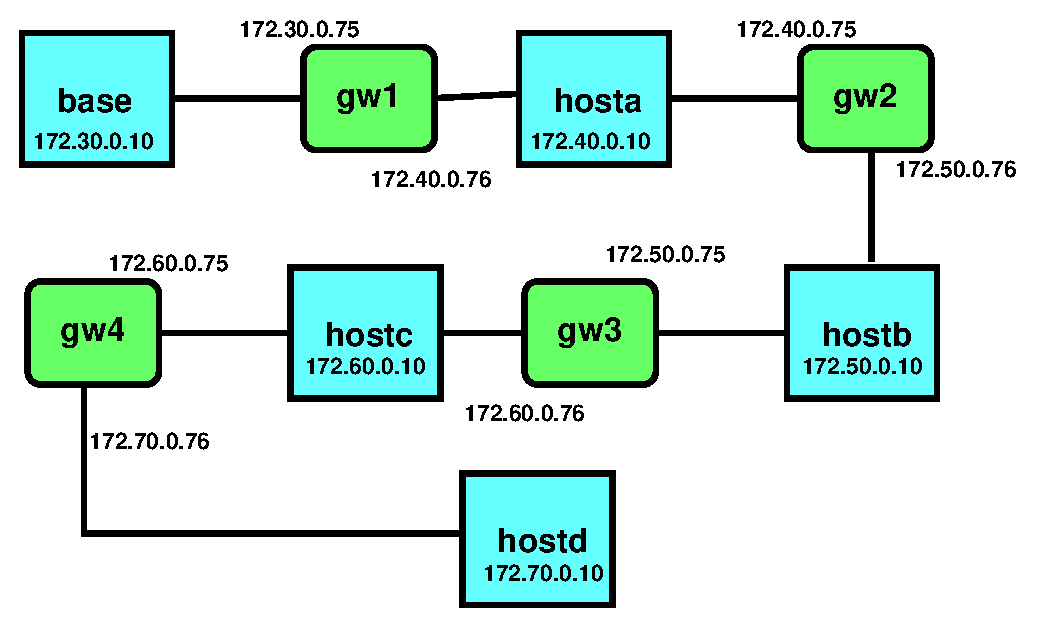
\includegraphics[scale=0.9]{network}
  \caption{\label{fig:1} Lab Network}
\end{figure}  
\end{center}

The addresses on the routers are as described in the figure. You won't
be dealing with those addresses.

\section{Lab Tasks}

\subsection{Initial setup}
The lab is started from the Labtainer working 
directory on your host, e.g., a Linux VM with Labtainer installed.
From there, issue the command:
\begin{verbatim}
    labtainer ssh-tunnel
\end{verbatim}

The resulting terminal is connected to the \base computer. You do all
your work inside this terminal.  

We will create the tunnel by creating \ssh connections, step by step
from one host to the next.  We will do this in a way, so that we can
issue commands to \host{d} directly from the \base. When \host{d}
investigates its connections as part of its auditing, it will only see
an \ssh connection to \host{c}, IP address 172.60.0.10, which would
probably be expected.

\subsection{Trying to Access the hosts}

Just to check, you should try to ping hosts \host{a}
$\ldots$ \host{d} and the gateways, to determine which devices
are visible from the \base host. You could use IP addresses or host
names to test. 

\subsection{Testing the Environment}
You should probably look at the documentation of \ssh using the command: 
\begin{verbatim}
man ssh
\end{verbatim}
The documentation is extensive. There are a lot of options.  You
should concentrate on the \verb|-f|, \verb|-4| and the \verb|-L|
options. These are the ones we will use.  If you are familiar with
\ssh, you may not have seen the \verb|-4| option.  This version of
\ssh support IPV6 and will attempt to use that unless the \verb|-4|
(use IPV4) is specified.  We are not using IPV6 so we need the
\verb|-4|.

From above you should have determined that \base can access
\host{a}.  Our reconnaissance has determined that \host{a}
has an \ssh server running so we will set up an \ssh connection to
\host{a}, just to test things out. Try the following commands:
\begin{verbatim}
ssh -4 hosta
\end{verbatim}
You will need to ``allow'' the connection and enter a user name and
password (see above) to log into \host{a}.

You should then issue the following command on \host{a} to get a sense
of its environment.
\begin{verbatim}
route -n
ping hostb
netstat -n | head
ps -ax | grep ssh
cat /etc/hosts
\end{verbatim}
The \textit{route} command will show you the routes the host knows.
The \textit{netstat} command will show you the current connections and
port numbers. The \textit{ps} command will show you the \ssh
connections (via the filter \textit{grep}).  
You will need to stop the \ping with \texttt{<CTRL-C>}.  You could try
pinging other hosts either by name or by IP address to see what is
connected. When you are done, you can ``leave'' \host{b} via:
\begin{verbatim}
exit
\end{verbatim}
which terminates the shell on \host{b}.  You should see from the
prompt that you are no typing at \base. 
\subsection{Creating First Step for Tunnel }
To set up the first leg of the tunnel, you should issue the command:
\begin{verbatim}
ssh -4 -f -L 1111:hostb:22 hosta -N
\end{verbatim}
Here are the descriptions and rational for the arguments:
\begin{description}
\item[\texttt{-4}]   As mentioned above, we are not using IPV6
  so we tell \ssh that we are using IPV4.

\item[\texttt{-f}]  This argument says that we are setting up an \ssh
  connection that will \textbf{NOT} connected to the terminal.  It
  will run in background mode.

\item[\texttt{hosta}] We skipped to nearly the end of the command
  because this \ssh actually directly connects to \host{a}.

\item[\texttt{-L 1111:hostb:22}] This argument is the ``trick'' in
  creating the first (and subsequent) legs of the tunnel.  In this
  case, it says:
  \begin{quotation}
    On \host{a}, the destination of the \ssh command, create an \ssh
    connection from \host{a} to port 22 on \host{b}.  Assign the TCP
    port \texttt{1111}  on \textbf{\base} to reference this connection.
  \end{quotation}
  The result is that when \base makes an \ssh connection to port
  \texttt{1111} it is actually communicating with \host{b},
  transparently through \host{a}.\footnote{For those of you with some
    \textit{Unix} background, we access this tunnel on localhost, IP
    address \texttt{127.0.0.1} and port \texttt{1111}.}

\item[\texttt{-N}] Do not execute a command on the remote host.
  Normally \ssh expects a command as the last set of arguments.
  the \verb|-N| arguments tells \ssh that this is a tunnel.

\end{description}

To tests the result of the command, the creation of the first leg of
the tunnel, you should try the command:
\begin{verbatim}
ssh -4 -p 1111 localhost
\end{verbatim}
The \verb|-p 1111| argument tells \ssh that it should connect to port
\texttt{1111} and the \texttt{localhost} argument says that that port
is on the \texttt{localhost}, in this case, \base.

Again, what is happening is that you have {\ssh}ed to the port
\texttt{1111} on the local host.  From the previous command the port
is connected through \host{a} to \host{b}.

You should figure out which host your terminal is now connected
to. You can tell by the \textit{prompt}.
Issue the commands we listed above and note which hosts are associated
with the \ssh connection.  You can tell that in the \textit{netstat}
command, one of the ports is \texttt{22}.

When you are done experimenting, you can type
\begin{verbatim}
exit
\end{verbatim}
Your prompt should now indicate that you are back typing to the \base host.

\subsection{Next Step in the Tunnel}
Now type the command:
\begin{verbatim}
ssh -4 -f -p 1111 -L 2222:hostc:22 localhost -N
\end{verbatim}
\label{cmd:step2}
As above, you should 

The port \texttt{1111} on the local host (hostname: \textit{localhost}) is
connected (from the First Step Command) to the \ssh port \texttt{22} on
\host{b}.  So typing an \ssh command on the local host is in effect,
telling \host{b} to make that connection. Since the \ssh command
is going through the tunnel from \base to \host{b},  the \texttt{2222}
port number will be a port on \base. 


\textbf{As a result, any \ssh command on \base using the port number
  \texttt{2222} will be directed at \host{c}}.

Now, using port \texttt{2222}, \ssh to \host{c} and experiment as
above. 

\subsection{Third Step in the Tunnel}

It is your job to now figure out and execute the \ssh command that
connects port \texttt{3333} on localhost (\base) to the \ssh port on \host{d}.
You should mimic the command in \ref{cmd:step2}.

Once you have made the tunnel connection to \host{d} you should try
logging into \host{d} and explore as you did before.  Note that
\host{d} will not have a direct connection to either \base or \host{b}.

\subsection{``Proving'' You Made the Tunnel}
You now need to provide to the automagic lab grader that you have, in
fact make the tunnel. To do that we have provided a file,
\textbf{copyfile.txt} on \host{d}.  You should copy this file over the
tunnel to \base.  To do that you can use the \scp command, copy a file
over an \ssh tunnel. Here is the command:
\begin{verbatim}
scp -P 3333 localhost:copyfile.txt /home/ubuntu
\end{verbatim}
Note that the port is identified with a capital \textbf{\texttt{P}}.
The \texttt{/home/ubuntu} is the home directory where you should have
seen the \texttt{copyfile.txt} file when you were looking in \host{d}
above.

When using \scp, normally one would say something like
\verb|remotehostname:filename| to identify a file on the remote host
to copy.  We are, in fact doing the same thing here. Port
\texttt{3333} on localhost, in this case, refers to \host{d}, so
\verb|-P 3333 localhost:copyfile.txt| refers to \texttt{copyfile.txt}
in the home directory of the user \textit{ubuntu} on \host{d}.

You can check that the file was copied using the command:
\begin{verbatim}
ls -l
\end{verbatim}
It should appear in the listing.  If it is there, you can look at its
contents with the command:
\begin{verbatim}
less copyfile.txt
\end{verbatim}
which will write the contents of the not very interesting file to
\textit{stdout}, the terminal window.


\subsection{Stopping the Lab}
Be sure to stop the lab with the command
\begin{verbatim}
stoplab
\end{verbatim}
in the same terminal window you issued the \verb|labtainer| command.

We need this, since this will save much of your output, and the
automagic grader will be able to determine whether you were successful
or not.

\section{Final Thoughts}
We have used port \texttt{22} as our final destination port on \host{d}.
The reason is that we want to copy files from \host{d} to \base.  If
we wanted to access a web server on \host{d} we could have used a
a destination port of say \texttt{443} on the final stage of our
tunnel instead of \texttt{22}.  To access the web server we would use
the \textit{url}:
\begin{verbatim}
https://localhost:3333
\end{verbatim}
in our local web browser. The same idea would work for other services.
We only need \ssh for the intermediate legs of the tunnel. 
\end{document}

